%
%%%%%%%%%%%%%%%%%%%%%%%%%%%%%%%%%%%%%%%%%%%%%%%%%%%%%%%%%%%%%%%%%%%%%%%%
\chapter{CUE}
%%%%%%%%%%%%%%%%%%%%%%%%%%%%%%%%%%%%%%%%%%%%%%%%%%%%%%%%%%%%%%%%%%%%%%%%
%
The CUE is the bug/development tracker of \telemacsystem.
It is available at the following address \url{cue.opentelemac.org}.
In order to login use your SVN login and password.
%
%
\section{Projects}
%
%
\label{proj}
It is divided in multiple projects:
\begin{itemize}
\item Modules: Those are the modules in the \telemacsystem code.
\item Sites: This concern all the development tools (CUE, CIS, Website...).
\item Supporting scripts: This concerns all the environment scripts (Python and
Perl) as well as parallelism, the automatic installer and the Inputs and
Outputs.
\end{itemize}
\begin{figure}[H]
    \centering
    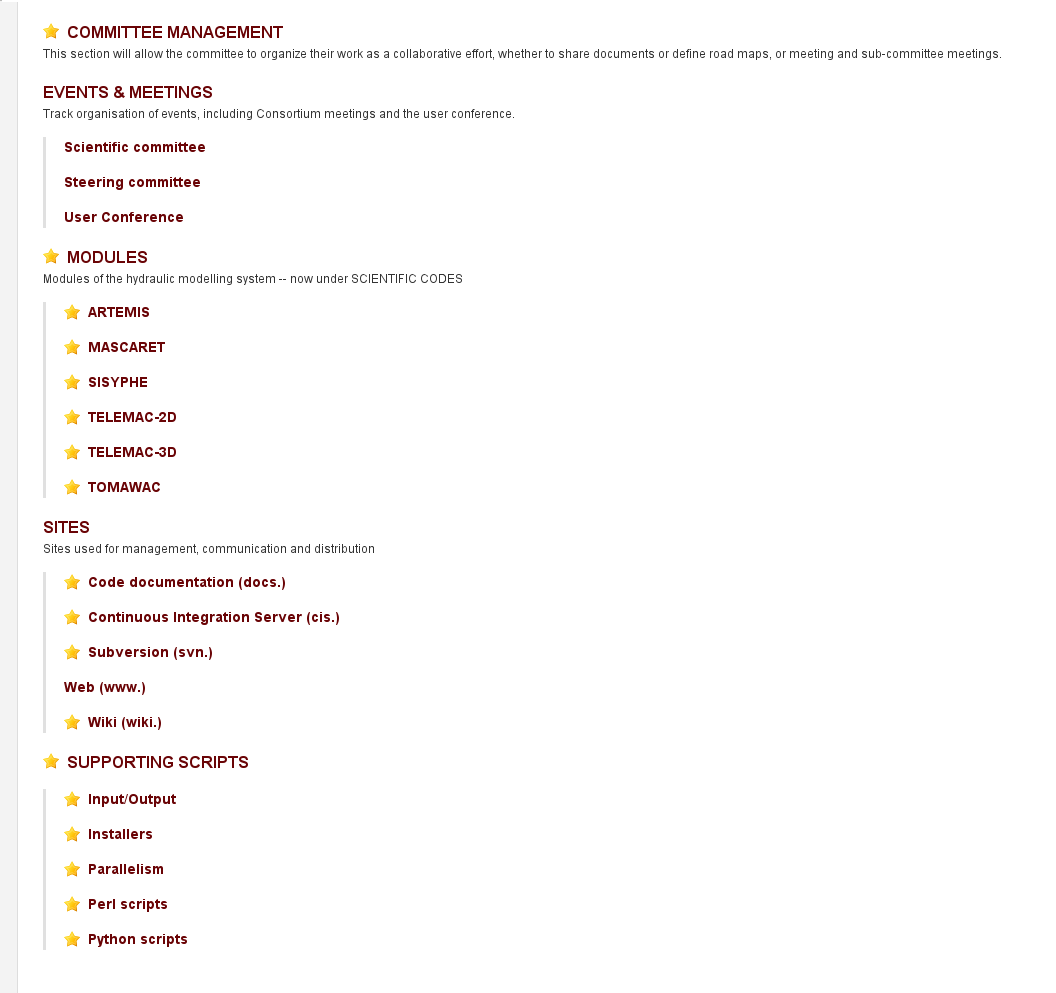
\includegraphics[scale=0.35]{graphics/cue-projects.png}
    \caption{CUE projects}
    \label{fig:cue-projects}
\end{figure}
%
%
\section{Create a ticket}
%
%
To add a new ticket you must go into the project your ticket concern and add
click on "New issue". This will lead you to the page shown on Fig
\ref{fig:cue-ticket}.  You will then need to fill the following information:
\begin{itemize}
\item Tracker: type of the ticket (Bug, Feature, Documentation,
Validation/Verif/Application).
\item Subject: Title of the ticket.
\item Description: Give an full explication of the problem.
\item Status: Status of the ticket (Set to new on creation).
\item Priority: Urgency of the ticket.
\item Assignee: Person in charge of the development integration.
\item Category: Category of the work.
\item Target Version: Version of the code in which the development should be
integrated.
\item Watchers: People that will get an update every time the ticket is
modified.
\end{itemize}
\begin{figure}[H]
    \centering
    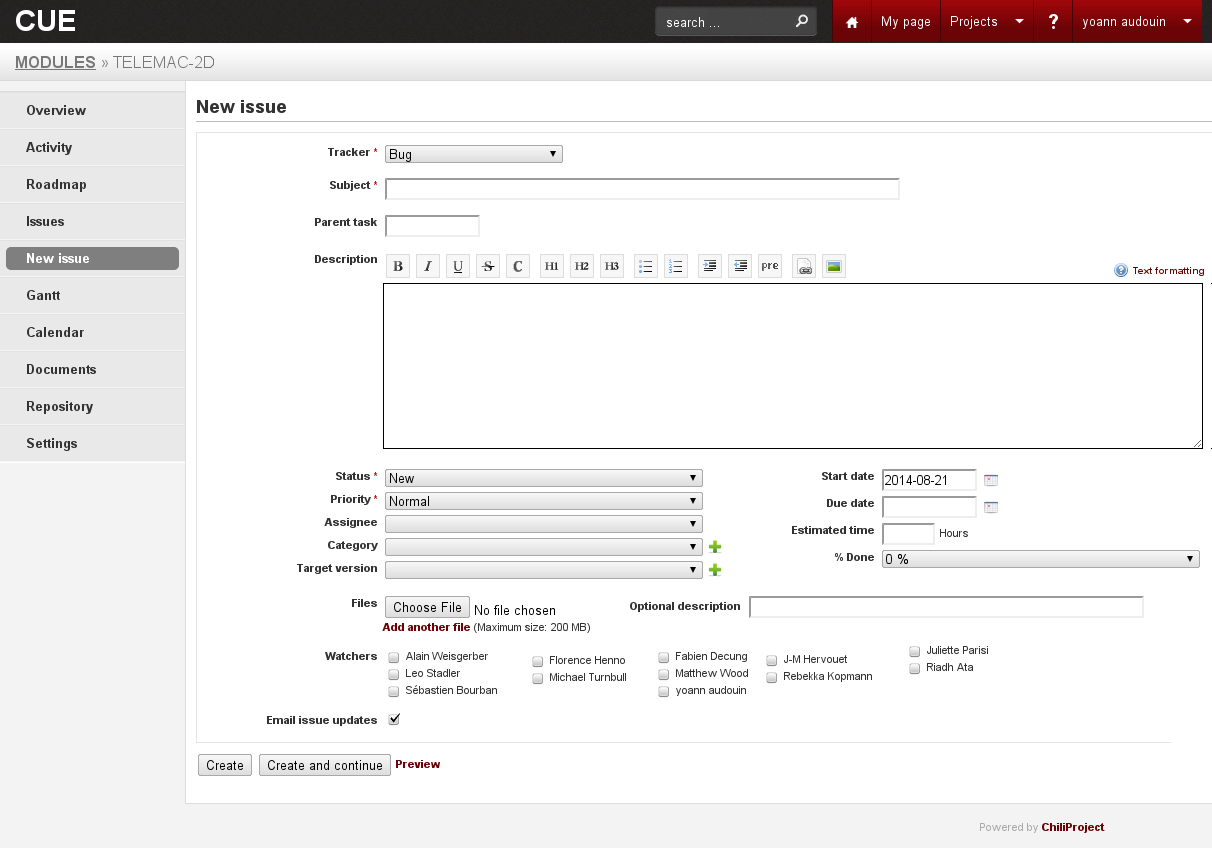
\includegraphics[scale=0.35]{graphics/cue-ticket.png}
    \caption{Creation of a ticket}
    \label{fig:cue-ticket}
\end{figure}

\begin{WarningBlock}{Warning:}
If you do not see the "New issue" button then you forgot to ask in the email
(described in Section \ref{mail}) the project you are working on, you will need
to send a new one to be see that button.
\end{WarningBlock}
%
%
\section{Modify a ticket}
%
%
To Modify a ticket go into the project your ticket is in then click on the
ticket and on the ticket page click on the "update" button in the upper right
corner of the page. The Fig \ref{fig:cue-modify} shows the page you get when
clicking on a ticket.

You will have to update your ticket as your work advance, either by adding
comments on what you have done or by changing its status. For example a bug is
set to "resolved" once we found its solution and set to "closed" once the
correction is integrated in the main version.
%
\begin{figure}[H]
    \centering
    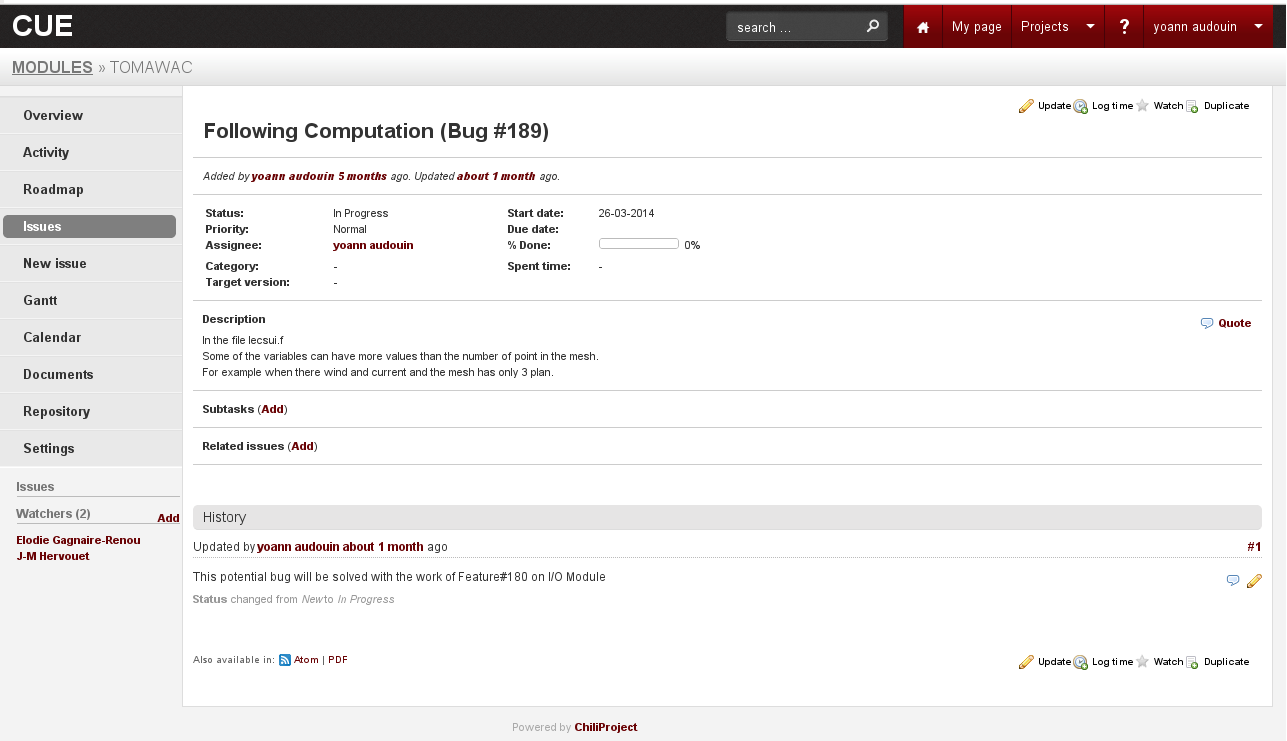
\includegraphics[scale=0.35]{graphics/cue-modify.png}
    \caption{Modification of a ticket}
    \label{fig:cue-modify}
\end{figure}
